%%%%%%%%%%%%%%%%%%%%%%%%%%%%%%%%%%%%%%%%%%%%%%%%%%%%%%%%%%%%%%%%%%%%%%%%%%%%%%%%%%%%
%%%%%%%%%%%          Preamble
%%%%%%%%%%%%%%%%%%%%%%%%%%%%%%%%%%%%%%%%%%%%%%%%%%%%%%%%%%%%%%%%%%%%%%%%%%%%%%%%%%%% 
\documentclass[9pt]{beamer}
\usepackage{setspace}
\usepackage{color}
\usepackage{amsmath,lmodern}
\usepackage{hyperref}
\usepackage{graphicx}
\usepackage{multirow}
\usepackage{bm}
\usepackage{graphicx}
\usepackage{subfig}
\usepackage[textfont={scriptsize}]{caption}
\usepackage{tikz}
\usetikzlibrary{fit,shapes.misc}
\usepackage{pdflscape}
\usepackage{amsmath}
\usepackage{lscape}
\usepackage{enumerate}
\usepackage{epstopdf}
\usepackage{appendixnumberbeamer}
\usepackage{bigints}
\usepackage{booktabs}
\usepackage{color,soul}
\usepackage{grffile}
\usepackage{relsize}
\newcounter{nodemarkers}
\usepackage{tikz}
\newcommand{\toplinesmall}{%
  \tikz[remember picture,overlay] {%
    \draw[blue,thick] ([yshift=-.9cm, xshift=.9cm]current page.north west)
             -- ([yshift=-.9cm,xshift=3.6cm]current page.north west);}}
             
\newcommand{\toplinemedium}{%
  \tikz[remember picture,overlay] {%
    \draw[blue,thick] ([yshift=-.9cm, xshift=.9cm]current page.north west)
             -- ([yshift=-.9cm,xshift=6.2cm]current page.north west);}}
 
 \newcommand{\toplinelarge}{%
  \tikz[remember picture,overlay] {%
    \draw[blue,thick] ([yshift=-.9cm, xshift=.9cm]current page.north west)
             -- ([yshift=-.9cm,xshift=8.9cm]current page.north west);}}           
             
 \newcommand{\toplinexlarge}{%
  \tikz[remember picture,overlay] {%
    \draw[blue,thick] ([yshift=-.9cm, xshift=.9cm]current page.north west)
             -- ([yshift=-.9cm,xshift=12cm]current page.north west);}}                       
             
\setbeamertemplate{footline}
{
  \leavevmode%
  \hbox{%
  \begin{beamercolorbox}[wd=.333333\paperwidth,ht=2.25ex,dp=1ex,center]{author in head/foot}%
    \usebeamerfont{author in head/foot}{\textcolor{blue}{ECON712}}
  \end{beamercolorbox}%
  \begin{beamercolorbox}[wd=.333333\paperwidth,ht=2.25ex,dp=1ex,center]{title in head/foot}%
    \usebeamerfont{title in head/foot}{\textcolor{blue}{Winter 2026}}
  \end{beamercolorbox}%
  \begin{beamercolorbox}[wd=.333333\paperwidth,ht=2.25ex,dp=1ex,right]{date in head/foot}%
    \usebeamerfont{date in head/foot}{\textcolor{blue}{Lectures 13 \: \: \: \: \: \: \: }
    \insertframenumber{} / \inserttotalframenumber\hspace*{2ex}} 
  \end{beamercolorbox}}%
  \vskip0pt%
}
\newtheorem{proposition}[theorem]{Proposition}

\newcommand\marktopleft[1]{%
    \tikz[overlay,remember picture] 
        \node (marker-#1-a) at (-0.2,1.2ex) {};%
}
\newcommand\markbottomright[1]{%
    \tikz[overlay,remember picture] 
        \node (marker-#1-b) at (0.16,-1ex) {};%
    \tikz[overlay,remember picture,thick,inner sep=4pt]
        \node[draw,rectangle,rounded corners, blue, fit=(marker-#1-a.center) (marker-#1-b.center)] {};%
}

\setbeamertemplate{itemize items}[ball]
\setbeamertemplate{itemize subitem}[triangle]
\setbeamertemplate{itemize subsubitem}[triangle]
\beamertemplatenavigationsymbolsempty
\addtobeamertemplate{frametitle}{\vspace*{0.19cm}}{\vspace*{0cm}}



%%%%%%%%%%%%%%%%%%%%%%%%%%%%%%%%%%%%%%%%%%%%%%%%%%%%%%%%%%%%%%%%%%%%%%%
%%%%%%%%%%%%%%%%%%%%%%%%%%%%%%%%%%%%%%%%%%%%%%%%%%%%%%%%%%%%%%%%%%%%%%% 
%%%%%%%%%  									    Define Title									                                       %%%%%%%%%
%%%%%%%%%%%%%%%%%%%%%%%%%%%%%%%%%%%%%%%%%%%%%%%%%%%%%%%%%%%%%%%%%%%%%%%
%%%%%%%%%%%%%%%%%%%%%%%%%%%%%%%%%%%%%%%%%%%%%%%%%%%%%%%%%%%%%%%%%%%%%%% 
\title{ECON 712: Applied Econometrics} 
\author{Lecture 13: Potential Outcomes and Causality}
\date{}
\AtBeginSection[]
{
 \begin{frame}<beamer>
 \tableofcontents[currentsection]
 \end{frame}
}



%%%%%%%%%%%%%%%%%%%%%%%%%%%%%%%%%%%%%%%%%%%%%%%%%%%%%%%%%%%%%%%%%%%%%%%
%%%%%%%%%%%%%%%%%%%%%%%%%%%%%%%%%%%%%%%%%%%%%%%%%%%%%%%%%%%%%%%%%%%%%%% 
%%%%%%%% 						     				Document								                                                %%%%%%%%
%%%%%%%%%%%%%%%%%%%%%%%%%%%%%%%%%%%%%%%%%%%%%%%%%%%%%%%%%%%%%%%%%%%%%%%
%%%%%%%%%%%%%%%%%%%%%%%%%%%%%%%%%%%%%%%%%%%%%%%%%%%%%%%%%%%%%%%%%%%%%%% 
\begin{document}
\setbeamercovered{transparent}


\begin{frame}
\maketitle
\end{frame}

\begin{frame}
\frametitle{\: \: \: E.g. Sorting on Unobservables}
\toplinemedium
\begin{itemize}
    \item Suppose we have data on two internationally students observationally equivalent ($i=M, K$):
    \begin{itemize}
        \vspace{0.08in}
        \item $D_i=1$ if student $i$ buys insurance (\textit{treatment} group), $D_i=0$ if student $i$ does not buy insurance (\textit{control} group)
        \vspace{0.08in}
        \item $Y_{1i}$: health outcome of student $i$ if s/he buys insurance, $Y_{0i}$: health outcome of student $i$ if s/he does not buy insurance
    \end{itemize}
    \vspace{0.11in}
    \item A causal effect of the policy would be equivalent to $Y_{1i}-Y_{0i}$ for either $i=M$ or $i=K$
    \begin{itemize}
        \vspace{0.08in}
        \item Using the following table, we show that a simple empirical comparison leads to imprecise estimates of the causal effect:
        \begin{figure}
        \centering
        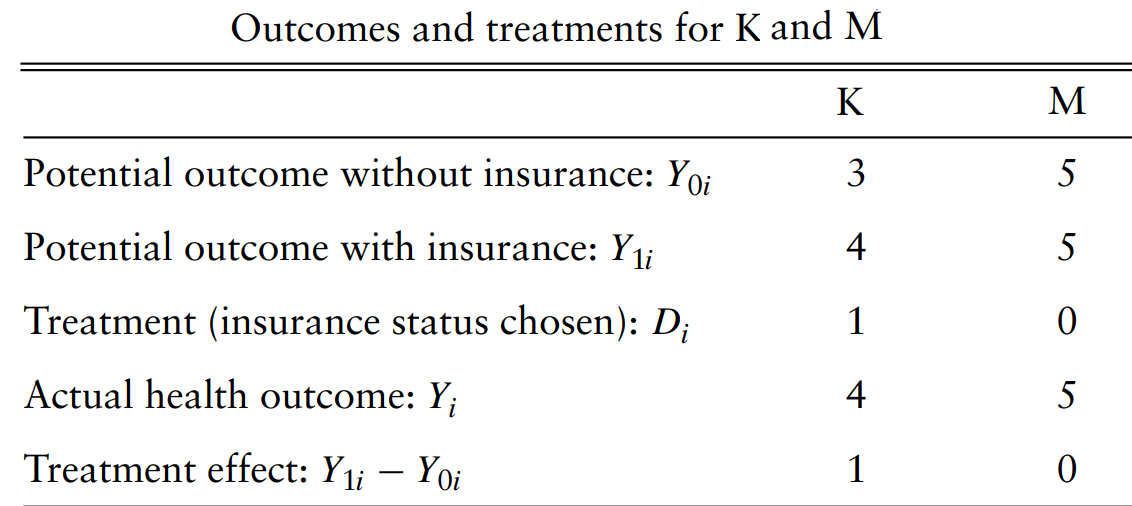
\includegraphics[scale=0.3]{health_student}
        \end{figure}
    \end{itemize}
\end{itemize}
\end{frame}


\begin{frame}
\frametitle{\: \: \: Average Treatment Effect}
\toplinemedium
\begin{block}{Definition: Average Treatment Effect (ATE)}
    The average treatment effect is the population average of all $i$ individual treatment effects
\end{block}
\vspace{0.11in}
\begin{eqnarray*}
    E[\delta_i] \: = \: E[Y_{1i} - Y_{0i}] \: = \: E[Y_{1i}] - E[Y_{0i}]
\end{eqnarray*}
\vspace{0.08in}
\begin{itemize}
    \item Cannot be calculated because $Y_{1i}$ and $Y_{0i}$ do not exist \textit{for the same unit}
\end{itemize}
\end{frame}


\begin{frame}
\frametitle{\: \: \: Average Treatment Effect dgd on the Treated}
\toplinelarge
\begin{block}{Definition: Average Treatment Effect on the Treated (ATT)}
    The average treatment effect on the treatment group is equal to the average treatment effect conditional on being a treatment group member:
\end{block}
\vspace{0.08in}
\begin{eqnarray*}
    E[\delta_i \mid D=1] \: = \: E[Y_{1i} - Y_{0i} \mid D=1] \: = \: E[Y_{1i} \mid D=1] - E[Y_{0i} \mid D=1]
\end{eqnarray*}
\vspace{0.08in}
\begin{itemize}
    \item Cannot be calculated because $Y_{1i}$ and $Y_{0i}$ do not exist \textit{for the same unit}
\end{itemize}
\end{frame}


\begin{frame}
\frametitle{\: \: \: Average Treatment Effect on the Untreated}
\toplinelarge
\begin{block}{Definition: Average Treatment Effect on the Untreated (ATU)}
    The average treatment effect on the untreated group is equal to the average treatment effect conditional on being untreated:
\end{block}
\vspace{0.08in}
\begin{eqnarray*}
    E[\delta_i \mid D=0] \: = \: E[Y_{1i} - Y_{0i} \mid D=0] \: = \: E[Y_{1i} \mid D=0] - E[Y_{0i} \mid D=0]
\end{eqnarray*}
\vspace{0.08in}
\begin{itemize}
    \item Cannot be calculated because $Y_{1i}$ and $Y_{0i}$ do not exist \textit{for the same unit}
\end{itemize}
\end{frame}


\begin{frame}
\frametitle{\: \: \: Independence}
\toplinesmall
\begin{block}{Independence Assumption}
    Treatment is assigned to a population independent of that population's potential outcomes:
    \begin{eqnarray*}
        (Y_{0i}, Y_{1i}) \perp\!\!\!\perp D_i
    \end{eqnarray*}
\end{block}
\vspace{0.08in}
\begin{itemize}
    \item This is random or quasi-random assignment and ensures mean potential outcomes for the treatment group and control group are the same. Also ensures other variables are distributed the same for a large sample:
    \begin{eqnarray*}
        E[Y_{0i} \mid D=1] \: = \: E[Y_{0i} \mid D=0] \\[-4pt]
        E[Y_{1i} \mid D=1] \: = \: E[Y_{1i} \mid D=0]
    \end{eqnarray*}
\end{itemize}
\end{frame}


\begin{frame}
\frametitle{\: \: \: Random Assignment}
\toplinemedium
\begin{eqnarray*}
\underbrace{E[y_i \mid d_i=1] - E[y_i \mid d_i=0]}_{\text{SDO}} &=&
    \underbrace{E[Y_{1i}] - E[Y_{0i}]}_{\text{Average Treatment Effect}} \\[6pt]
    && + \: \underbrace{E[Y_{0i} \mid D=1] - E[Y_{0i} \mid D=0]}_{\text{Selection bias}} \\[6pt]
    && + \: \underbrace{(1-\pi)(\text{ATT} - \text{ATU})}_{\text{Heterogeneous treatment effect bias}}
\end{eqnarray*}
\vspace{0.08in}
\begin{itemize}
    \item If treatment is independent of potential outcomes, then:
    \begin{eqnarray*}
        E[Y_{0i} \mid D=1] - E[Y_{0i} \mid D=0] = 0
    \end{eqnarray*}
\end{itemize}
\end{frame}


\begin{frame}
\frametitle{\: \: \: Random Assignment}
\toplinemedium
\begin{itemize}
    \item How does randomization eliminate heterogeneous treatment effect bias? Rewrite ATT and ATU:
    \begin{eqnarray*}
        \text{ATT} &=& E[Y_{1i} \mid D=1] - E[Y_{0i} \mid D=1] \\
        \text{ATU} &=& E[Y_{1i} \mid D=0] - E[Y_{0i} \mid D=0]
    \end{eqnarray*}
    \vspace{0.05in}
    \item Under independence, rewrite $\text{ATT} - \text{ATU}$:
    \begin{eqnarray*}
        \text{ATT} - \text{ATU} &=& \mathbf{E[Y_{1i} \mid D=1]} - E[Y_{0i} \mid D=1] \\
                                 && - \: \mathbf{E[Y_{1i} \mid D=0]} + E[Y_{0i} \mid D=0] \: = \: 0
    \end{eqnarray*}
    \vspace{0.05in}
    \item Therefore, if treatment is independent of potential outcomes:
    \begin{eqnarray*}
        E[y_i \mid D_i=1] - E[y_i \mid D_i=0] \: = \: E[Y_{1i}] - E[Y_{0i}] \qquad \Rightarrow \qquad \text{SDO} = \text{ATE}
    \end{eqnarray*}
\end{itemize}
\end{frame}


\begin{frame}
\frametitle{\: \: \: ATE and Regression}
\toplinelarge
\begin{itemize}
    \item Define the following regression:
    \begin{eqnarray*}
        y_i = \hat{\beta}_0 + \hat{\delta} \: D_i + \hat{\epsilon}_i
    \end{eqnarray*}
  \item In ECON312 you showed that the OLS estimator of $\delta$ in a sample is:
    \begin{eqnarray*}
        \hat{\delta} = \frac{1}{n_1}\mathlarger{\sum}_{i=1}^{n_1} y_i - \frac{1}{n_0}\mathlarger{\sum}_{i=1}^{n_0} y_i
    \end{eqnarray*}

    \item From this equation, we obtain:
    \begin{eqnarray*}
    \underset{n_0,n_1\rightarrow \infty}{plim}\hat{\delta}=E[y_i \mid D_i=1] - E[y_i \mid D_i=0]\underbrace{=}_{(Y_{0i}, Y_{1i}) \perp\!\!\!\perp D_i}ATE
    \end{eqnarray*}
\vspace{0.08in}

\end{itemize}
\end{frame}

\begin{frame}
\frametitle{\: \: \: Randomization}
\toplinemedium
\begin{itemize}
\item We can also think about the independence assumption in the context of the population regression:
\begin{eqnarray*}
y_i=\underbrace{\beta_0}_{E[y_{0i}]}+\underbrace{\delta}_{E[y_{1i}-y_{0i}]} \: D_i+\underbrace{\epsilon_i}_{y_{0i}-E[y_{0i}]+(\delta_i-\delta)D_i}
\end{eqnarray*}
if randomly assigned:
\begin{eqnarray*}
E[y_{0i}|D_i=1]=E[y_{0i}|D_i=0]=E[y_{0i}]
\end{eqnarray*}
and additionally $E[\delta_i|D_i=1]=E[\delta_i]=\delta$ (ATT $=$ ATE), which together imply:
\begin{eqnarray*}
\begin{array}{lll}
E[\epsilon_i |D_i=0]&=&E[y_{0i}|D_i=0]-E[y_{0i}]=0 \\[2ex]
E[\epsilon_i |D_i=1]&=&\left(E[y_{0i}|D_i=1]-E[y_{0i}]\right) \\[2ex] 
                               &  &+\left(E[\delta_i|D_i=1]-\delta\right) \;=\;0 \\[2ex]
\underbrace{\Rightarrow}_{\text{LIE}} E[\epsilon_i]=0 & & 
\end{array}
\end{eqnarray*}

\item So the MM/OLS estimator is a consistent estimator of the \textbf{ATE}
\end{itemize}
\end{frame}


%%%%%%%%%%%%%%%%%%%%%%%%%%%%%%%%%%%%%%%%%%%%%%%%%%%%%%%%%%%%%%%%%%%%%%%
%%%%%%%%%%%%%%%%%%%%%%%%%%%%%%%%%%%%%%%%%%%%%%%%%%%%%%%%%%%%%%%%%%%%%%%
%%%%%%%%%              One Treatment with Controls
%%%%%%%%%%%%%%%%%%%%%%%%%%%%%%%%%%%%%%%%%%%%%%%%%%%%%%%%%%%%%%%%%%%%%%%
%%%%%%%%%%%%%%%%%%%%%%%%%%%%%%%%%%%%%%%%%%%%%%%%%%%%%%%%%%%%%%%%%%%%%%%

\begin{frame}
\frametitle{\: \: \: Limits of Independence}
\toplinemedium
\begin{itemize}
    \item Full independence $(Y_{0i}, Y_{1i}) \perp\!\!\!\perp D_i$ requires \textbf{randomized} treatment assignment
    \vspace{0.11in}
    \item In most observational data, treatment is \textbf{not} randomly assigned:
    \begin{itemize}
        \vspace{0.08in}
        \item Students who attend university self-select based on ability and family background
        \vspace{0.08in}
        \item Individuals who buy health insurance differ systematically from those who do not
        \vspace{0.08in}
        \item Firms that adopt a policy differ systematically from those that do not
    \end{itemize}
    \vspace{0.11in}
    \item Key question: can we make treatment ``as good as random'' \textit{after} conditioning on observed characteristics $\bm{X}_i$?
    \vspace{0.11in}
    \item \textbf{Conditional Independence Assumption (CIA)}:
    \begin{eqnarray*}
        (Y_{0i},\, Y_{1i}) \perp\!\!\!\perp D_i \mid \bm{X}_i
    \end{eqnarray*}
    \begin{itemize}
        \item Also called \textit{selection on observables}, \textit{unconfoundedness}, or \textit{ignorability}
        \vspace{0.05in}
        \item Requires \textbf{overlap}: $0 < P(D_i = 1 \mid \bm{X}_i) < 1$ (or a functional form assumption with within treatment group variation)
    \end{itemize}
\end{itemize}
\end{frame}


\begin{frame}
\frametitle{\: \: \: CIA: What It Buys You}
\toplinemedium
\begin{itemize}
    \item CIA implies that, \textbf{within cells defined by} $\bm{X}_i$, there is no selection bias, and ATT=ATU:
    \begin{eqnarray*}
        E[Y_{0i} \mid D_i=1,\, \bm{X}_i] \:=\: E[Y_{0i} \mid D_i=0,\, \bm{X}_i] \:=\: E[Y_{0i} \mid \bm{X}_i] \\
	  E[Y_{1i} \mid D_i=1,\, \bm{X}_i] \:=\: E[Y_{1i} \mid D_i=0,\, \bm{X}_i] \:=\: E[Y_{1i} \mid \bm{X}_i]	
    \end{eqnarray*}
    \vspace{0.03in}
    \item Therefore, the \textcolor{blue}{conditional} ATE is \textbf{identified} from observed data:
    \begin{eqnarray*}
        E[Y_i \mid D_i=1,\, \bm{X}_i] - E[Y_i \mid D_i=0,\, \bm{X}_i] \:=\: E[Y_{1i}-Y_{0i} \mid \bm{X}_i]
    \end{eqnarray*}
    \vspace{0.03in}

    \item \textbf{Importantly}: CIA does \textit{not} say treatment is random --- it says that \textit{all} variables that jointly determine $D_i$ and potential outcomes are \textbf{observed} in $\bm{X}_i$
    \vspace{0.05in}
    \item If \textbf{unobserved} confounders remain, CIA fails $\Rightarrow$ need IV, DiD, RD, \ldots
\end{itemize}
\end{frame}

\begin{frame}
\frametitle{\: \: \: ATT, ATU, and ATE}
\toplinemedium
\begin{itemize}
\item Three distinct parameters of interest, differing in the \textbf{population} over which we average:
\begin{eqnarray*}
\text{ATE} &=& \int E[Y_{1i}-Y_{0i}\mid \bm{X}_i=\bm{x}]\cdot f(\bm{x})\,d\bm{x} \\[2ex]
\text{ATT} &=& \int E[Y_{1i}-Y_{0i}\mid \bm{X}_i=\bm{x}]\cdot f(\bm{x}\mid D_i=1)\,d\bm{x} \\[2ex]
\text{ATU} &=& \int E[Y_{1i}-Y_{0i}\mid \bm{X}_i=\bm{x}]\cdot f(\bm{x}\mid D_i=0)\,d\bm{x}
\end{eqnarray*}
\vspace{0.03in}
\item ATT $\neq$ ATU because they \textbf{integrate over different distributions of} $\bm{X}_i$ (unless the treatment is homogeneous)
\vspace{0.03in}
\item ATE is a \textbf{weighted average} of ATT and ATU by the Law of Iterated Expectations:
\begin{eqnarray*}
\text{ATE} \:=\: P(D_i=1)\cdot\text{ATT} \:+\: P(D_i=0)\cdot\text{ATU}
\end{eqnarray*}
\item (Note, under \textbf{random assignment}: $f(x\mid D_i=1)=f(x\mid D_i=0)=f(x)$, so ATT $=$ ATU $=$ ATE)
\end{itemize}
\end{frame}

\begin{frame}
\frametitle{\: \: \: OLS with a binary Control: What Does Regression Identify?}
\toplinexlarge
\begin{itemize}
    \item Under CIA,  $y_i = \beta_0 + \delta^R \: D_i + \beta_1 A_i + u_i$
    \vspace{0.05in}
    \item With \textbf{heterogeneous} treatment effects $\delta_{A_i} \equiv E[y_{1i}-y_{0i}\mid A_i]$, then:
    \begin{eqnarray*}
    \delta^R=\frac{E[Var(D_i|A_i) \delta_{A_i}]}{E[Var(D_i|A_i)]}
  \end{eqnarray*}
  \item If $\delta_{A_i}=\delta$ for all $A_i$,  then $\delta^R=\delta=ATE$
  \vspace{0.03in}
  \item On the other hand, when effect is heterogeneous, the weighting is different
  \vspace{0.03in}
  \item Despite the less straightforward weighting, the estimate is considered causal as it is a weighted average of causal effects
 \begin{itemize}
 \vspace{0.03in}
 \item Differences between ATE and $\delta^R$ are small when the heterogeneity is small
 \end{itemize}
  \vspace{0.03in}
  \item Linear regression still a powerful tool, in particular, when the covariate is continuous as the linearity does not require overlap, but that the covariate varies within treatment
  \begin{itemize}
\vspace{0.03in}
  \item Nevertheless, the in the last few decades matching estimators that directly estimate $ATT$ and $ATE$ has become more popular due to its direct interpretability (more of this later, time permitting) 
  \end{itemize}
  
\end{itemize}
\end{frame}


\begin{frame}
\frametitle{\: \: \: Omitted Variable Bias}
\toplinemedium
\begin{itemize}
    \item Suppose the \textbf{true} population model includes a confounder $X_i$:
    \begin{eqnarray*}
        y_i = \beta_0 + \delta \: D_i + \beta_1 X_i + u_i, \qquad E[u_i \mid D_i, X_i]=0
    \end{eqnarray*}
    \item If we \textbf{omit} $X_i$ and estimate $y_i = \hat{\beta}_0 + \hat{\delta} \: D_i + \hat{\epsilon}_i$, and, $\text{Cov}(X_i,D_i)\neq 0$, then $\text{Cov}(\epsilon_i,D_i)\neq 0$ and OLS is \textbf{inconsistent}:
    \begin{eqnarray*}
        \underset{n\rightarrow\infty}{plim}\;\hat{\delta} \;=\; \delta + \beta_1 \underbrace{\frac{\text{Cov}(X_i,D_i)}{\text{Var}(D_i)}}_{\equiv\,\gamma_1}
    \end{eqnarray*}
    where $\gamma_1$ is the slope from the auxiliary regression $X_i = \gamma_0 + \gamma_1 D_i + v_i$
    \item The bias $\beta_1\gamma_1$ has sign determined by: (i) whether $X_i$ raises $y_i$ ($\beta_1 \gtrless 0$) and (ii) whether treated units have higher $X_i$ ($\gamma_1 \gtrless 0$)
\vspace{0.03in}
    \item \textbf{Solution}: control for $X_i$ directly $\Rightarrow$ under CIA, OLS on the long regression identifies $\delta$
\end{itemize}
\end{frame}


%%%%%%%%%%%%%%%%%%%%%%%%%%%%%%%%%%%%%%%%%%%%%%%%%%%%%%%%%%%%%%%%%%%%%%%
%%%%%%%%%%%%%%%%%%%%%%%%%%%%%%%%%%%%%%%%%%%%%%%%%%%%%%%%%%%%%%%%%%%%%%%
%%%%%%%%%                    Bad Controls
%%%%%%%%%%%%%%%%%%%%%%%%%%%%%%%%%%%%%%%%%%%%%%%%%%%%%%%%%%%%%%%%%%%%%%%
%%%%%%%%%%%%%%%%%%%%%%%%%%%%%%%%%%%%%%%%%%%%%%%%%%%%%%%%%%%%%%%%%%%%%%%

\begin{frame}
\frametitle{\: \: \: Bad Controls}
\toplinesmall
\begin{itemize}
\item As is the case with omitted variable bias, adding \textcolor{blue}{bad} controls in the regression leads to inconsistent causal estimates
\vspace{0.11in}
\item A \textbf{bad control} is usually a variable that is itself an \textit{outcome} of the treatment, and adding it to the regression results in the following
\begin{enumerate}
\vspace{0.11in}
\item It \textbf{blocks part of the causal channel} you are trying to measure, which changes the interpretation of the causal estimate
\vspace{0.11in}
\item If the control does not satisfies the CIA, it introduces selection bias even if CIA or unconditional independence holds for the specification without the control
\end{enumerate}
\vspace{0.11in}
\item When 2. happens, MHE refers to this control as a \textbf{bad control}
\vspace{0.11in}
\begin{itemize}
\item \textbf{Bottom line}: when uncertain whether a control is good or bad, ask --- \textit{``Could the treatment change this variable?''} If yes, either think carefully about what the introduction of this variable does to the regression, or leave it out.
\end{itemize}
\end{itemize}
\end{frame}


\begin{frame}
\frametitle{\: \: \: Bad Controls: The Formal Argument}
\toplinelarge
\begin{itemize}
    \item Suppose $Y_i$ is wages, $D_i$ is university degree (treatment), and $W_i$ is white collar occupation.
   \begin{itemize}
   \vspace{0.11in}
   \item Assume that $Y_{D_i=0,i}, Y_{D_i=1,i} \perp\!\!\!\perp D_i$ so that the `short' regression, identifies a causal effect:
   \begin{eqnarray*}
   \begin{array}{lll}
   Y_i=\beta_0+\delta^{ATE} \: D_i+\epsilon &,& E[\epsilon_i|D_i]=E[\epsilon_i] 
   \end{array}
   \end{eqnarray*}
   \vspace{0.11in}
   \item Assume that $Y_{W_i=0,i}, Y_{W_i=1,i} \not \perp\!\!\!\perp W_i|D_i$ so that the `long' regression, introduces selection bias:  
    \begin{eqnarray*}
    \begin{array}{lll}
        Y_i \:=\beta_0+\delta^{R} \: D_i+\beta_1 \: W_i+\: u_i &,& E[u_i|D_i, W_i]\neq E[u_i] 
    \end{array}
    \end{eqnarray*}
  \end{itemize}
  \end{itemize}
\end{frame}



\end{document}


